\documentclass[noauthor,nooutcomes,handout,hints]{../ximera}

\graphicspath{  
{./}
{./whoAreYou/}
{./drawingWithTheTurtle/}
{./bisectionMethod/}
{./circles/}
{./anglesAndRightTriangles/}
{./lawOfSines/}
{./lawOfCosines/}
{./plotter/}
{./staircases/}
{./pitch/}
{./qualityControl/}
{./symmetry/}
{./nGonBlock/}
}


%% page layout
\usepackage[cm,headings]{fullpage}
\raggedright
\setlength\headheight{13.6pt}


%% fonts
\usepackage{euler}

\usepackage{FiraMono}
\renewcommand\familydefault{\ttdefault} 
\usepackage[defaultmathsizes]{mathastext}
\usepackage[htt]{hyphenat}

\usepackage[T1]{fontenc}
\usepackage[scaled=1]{FiraSans}

%\usepackage{wedn}
\usepackage{pbsi} %% Answer font


\usepackage{cancel} %% strike through in pitch/pitch.tex


%% \usepackage{ulem} %% 
%% \renewcommand{\ULthickness}{2pt}% changes underline thickness

\tikzset{>=stealth}

\usepackage{adjustbox}

\setcounter{titlenumber}{-1}

%% journal style
\makeatletter
\newcommand\journalstyle{%
  \def\activitystyle{activity-chapter}
  \def\maketitle{%
    \addtocounter{titlenumber}{1}%
                {\flushleft\small\sffamily\bfseries\@pretitle\par\vspace{-1.5em}}%
                {\flushleft\LARGE\sffamily\bfseries\thetitlenumber\hspace{1em}\@title \par }%
                {\vskip .6em\noindent\textit\theabstract\setcounter{question}{0}\setcounter{sectiontitlenumber}{0}}%
                    \par\vspace{2em}
                    \phantomsection\addcontentsline{toc}{section}{\thetitlenumber\hspace{1em}\textbf{\@title}}%
                     }}
\makeatother



%% thm like environments
\let\question\relax
\let\endquestion\relax

\newtheoremstyle{QuestionStyle}{\topsep}{\topsep}%%% space between body and thm
		{}                      %%% Thm body font
		{}                              %%% Indent amount (empty = no indent)
		{\bfseries}            %%% Thm head font
		{)}                              %%% Punctuation after thm head
		{ }                           %%% Space after thm head
		{\thmnumber{#2}\thmnote{ \bfseries(#3)}}%%% Thm head spec
\theoremstyle{QuestionStyle}
\newtheorem{question}{}



\let\freeResponse\relax
\let\endfreeResponse\relax

%% \newtheoremstyle{ResponseStyle}{\topsep}{\topsep}%%% space between body and thm
%% 		{\wedn\bfseries}                      %%% Thm body font
%% 		{}                              %%% Indent amount (empty = no indent)
%% 		{\wedn\bfseries}            %%% Thm head font
%% 		{}                              %%% Punctuation after thm head
%% 		{3ex}                           %%% Space after thm head
%% 		{\underline{\underline{\thmname{#1}}}}%%% Thm head spec
%% \theoremstyle{ResponseStyle}

\usepackage[tikz]{mdframed}
\mdfdefinestyle{ResponseStyle}{leftmargin=1cm,linecolor=black,roundcorner=5pt,
, font=\bsifamily,}%font=\wedn\bfseries\upshape,}


\ifhandout
\NewEnviron{freeResponse}{}
\else
%\newtheorem{freeResponse}{Response:}
\newenvironment{freeResponse}{\begin{mdframed}[style=ResponseStyle]}{\end{mdframed}}
\fi



%% attempting to automate outcomes.

%% \newwrite\outcomefile
%%   \immediate\openout\outcomefile=\jobname.oc
%% \renewcommand{\outcome}[1]{\edef\theoutcomes{\theoutcomes #1~}%
%% \immediate\write\outcomefile{\unexpanded{\outcome}{#1}}}

%% \newcommand{\outcomelist}{\begin{itemize}\theoutcomes\end{itemize}}

%% \NewEnviron{listOutcomes}{\small\sffamily
%% After answering the following questions, students should be able to:
%% \begin{itemize}
%% \BODY
%% \end{itemize}
%% }
\usepackage[tikz]{mdframed}
\mdfdefinestyle{OutcomeStyle}{leftmargin=2cm,rightmargin=2cm,linecolor=black,roundcorner=5pt,
, font=\small\sffamily,}%font=\wedn\bfseries\upshape,}
\newenvironment{listOutcomes}{\begin{mdframed}[style=OutcomeStyle]After answering the following questions, students should be able to:\begin{itemize}}{\end{itemize}\end{mdframed}}



%% my commands

\newcommand{\snap}{{\bfseries\itshape\textsf{Snap!}}}
\newcommand{\flavor}{\link[\snap]{https://snap.berkeley.edu/}}
\newcommand{\mooculus}{\textsf{\textbf{MOOC}\textnormal{\textsf{ULUS}}}}


\usepackage{tkz-euclide}
\tikzstyle geometryDiagrams=[rounded corners=.5pt,ultra thick,color=black]
\colorlet{penColor}{black} % Color of a curve in a plot



\ifhandout\newcommand{\mynewpage}{\newpage}\else\newcommand{\mynewpage}{}\fi


\title{The law of sines}
\author{Bart Snapp}

\begin{document}
\begin{abstract}
  The law of sines can help us draw triangles.
\end{abstract}
\maketitle

\begin{listOutcomes}
\item State the law of sines.
\item Explain why the law of sines is true.
\item Use the law of sines to solve a triangle.
\item Use the law of sines to write a \snap\ block that draws triangles
  based on the ASA congruence theorem.
\item Use the law of sines to write a \snap\ block that draws
  triangles based on the SAA congruence theorem.
\end{listOutcomes}

Given a triangle
\begin{center}
      \begin{tikzpicture}[geometryDiagrams]
        \coordinate (A) at (0,0);
        \coordinate (B) at (5,2);
        \coordinate (C) at (7,0);
        \tkzDrawSegment (A,B)
        \tkzDrawSegment (A,C)
        \tkzDrawSegment (C,B)
        \tkzLabelSegment[above left](A,B){$c$}
        \tkzLabelSegment[below](A,C){$b$}
        \tkzLabelSegment[above right](B,C){$a$}  

        \tkzMarkAngle[size=1.5cm,thin,mark=](C,A,B)
        \tkzLabelAngle[pos=1.2](C,A,B){$\alpha$}

        \tkzMarkAngle[size=0.8cm,thin,mark=](A,B,C)
        \tkzLabelAngle[pos=.5](A,B,C){$\beta$}

        \tkzMarkAngle[mark=,size=.9,thin](B,C,A)
        \tkzLabelAngle[pos=.6](B,C,A){$\gamma$}
        
      \end{tikzpicture}
\end{center}
the \textbf{law of sines} states
\[
\frac{a}{\sin(\alpha)} = \frac{b}{\sin(\beta)} = \frac{c}{\sin(\gamma)}.
\]


\mynewpage


\begin{question}
  We'll explain WHY the law of sines is true.
  \begin{enumerate}
  \item Use this picture
    \begin{center}
      \begin{tikzpicture}[geometryDiagrams]
        \coordinate (A) at (0,0);
        \coordinate (B) at (5,2);
        \coordinate (C) at (7,0);
        \tkzDrawSegment (A,B)
        \tkzDrawSegment (A,C)
        \tkzDrawSegment (C,B)
        \tkzLabelSegment[above left](A,B){$c$}
        %\tkzLabelSegment[below](A,C){$b$}
        \tkzLabelSegment[above right](B,C){$a$}  
        
        \tkzMarkAngle[size=1.5cm,thin,mark=](C,A,B)
        \tkzLabelAngle[pos=1.2](C,A,B){$\alpha$}

        %\tkzMarkAngle[size=0.8cm,thin,mark=](A,B,C)
        %\tkzLabelAngle[pos=.5](A,B,C){$\beta$}

        \tkzMarkAngle[mark=,size=.9,thin](B,C,A)
        \tkzLabelAngle[pos=.6](B,C,A){$\gamma$}
        \tkzDrawLine[altitude](A,B,C)\tkzGetPoint{D}
        \tkzMarkRightAngle[thin](B,D,C)
        \tkzLabelSegment[left](D,B){$h$}  
      \end{tikzpicture}
    \end{center}
    to explain why
    \[
    \frac{a}{\sin(\alpha)} = \frac{c}{\sin(\gamma)}.
    \]
    \item Now use this picture
    \begin{center}
      \begin{tikzpicture}[geometryDiagrams]
        \coordinate (A) at (0,0);
        \coordinate (B) at (5,2);
        \coordinate (C) at (7,0);
        \tkzDrawSegment (A,B)
        \tkzDrawSegment (A,C)
        \tkzDrawSegment (C,B)
        \tkzLabelSegment[below right](A,B){$c$}
        \tkzLabelSegment[below](A,C){$b$}
        %\tkzLabelSegment[above right](B,C){$a$}  

        %\tkzMarkAngle[size=1.5cm,thin,mark=](C,A,B)
        %\tkzLabelAngle[pos=1.2](C,A,B){$\alpha$}

        \tkzMarkAngle[size=0.8cm,thin,mark=](A,B,C)
        \tkzLabelAngle[pos=.5](A,B,C){$\beta$}

        \tkzMarkAngle[mark=,size=.9,thin](B,C,A)
        \tkzLabelAngle[pos=.6](B,C,A){$\gamma$}
        \tkzDrawLine[altitude](C,A,B)\tkzGetPoint{D}
        \tkzDrawSegment[dashed](D,B)
        \tkzMarkRightAngle[thin](C,D,A)
        \tkzLabelSegment[above left](D,A){$h$}  
      \end{tikzpicture}
  \end{center}
  to explain why
  \[
  \frac{b}{\sin(\beta)} = \frac{c}{\sin(\gamma)}.
  \]
  \begin{hint}
    Use the fact that $\sin(180-\theta) = \sin(\theta)$.
  \end{hint}
    \end{enumerate}
    
\begin{question}
\begin{enumerate}
 \item Explain how the previous problem proves the law of sines.
 \item Restate the Law of Sines in your own words. Use sentences and nonmath language as much as possible.
\end{enumerate}


\end{question}

  \begin{freeResponse}
    \begin{enumerate}
    \item If we look at the first picture:
      \begin{center}
      \begin{tikzpicture}[geometryDiagrams]
        \coordinate (A) at (0,0);
        \coordinate (B) at (5,2);
        \coordinate (C) at (7,0);
        \tkzDrawSegment (A,B)
        \tkzDrawSegment (A,C)
        \tkzDrawSegment (C,B)
        \tkzLabelSegment[above left](A,B){$c$}
        %\tkzLabelSegment[below](A,C){$b$}
        \tkzLabelSegment[above right](B,C){$a$}  
        
        \tkzMarkAngle[size=1.5cm,thin,mark=](C,A,B)
        \tkzLabelAngle[pos=1.2](C,A,B){$\alpha$}

        %\tkzMarkAngle[size=0.8cm,thin,mark=](A,B,C)
        %\tkzLabelAngle[pos=.5](A,B,C){$\beta$}

        \tkzMarkAngle[mark=,size=.9,thin](B,C,A)
        \tkzLabelAngle[pos=.6](B,C,A){$\gamma$}
        \tkzDrawLine[altitude](A,B,C)\tkzGetPoint{D}
        \tkzMarkRightAngle[thin](B,D,C)
        \tkzLabelSegment[left](D,B){$h$}  
      \end{tikzpicture}
    \end{center}
    We see that
    \begin{align*}
      \sin(\alpha) &= \frac{h}{c},\\
      \sin(\gamma) &= \frac{h}{a}.
    \end{align*}
    Now, in each equation above, solve for $h$, and set the other
    sides of the equations equal to each other:
    \[
    a\cdot \sin(\gamma)=c\cdot \sin(\alpha)
    \]
    Finally divide both sides by $\sin(\alpha)\sin(\gamma)$ to find
    \[
    \frac{a}{\sin(\alpha)} = \frac{c}{\sin(\gamma)}.
    \]

    \item For the second part, consider this picture:
    \begin{center}
      \begin{tikzpicture}[geometryDiagrams]
        \coordinate (A) at (0,0);
        \coordinate (B) at (5,2);
        \coordinate (C) at (7,0);
        \tkzDrawSegment (A,B)
        \tkzDrawSegment (A,C)
        \tkzDrawSegment (C,B)
        \tkzLabelSegment[below right](A,B){$c$}
        \tkzLabelSegment[below](A,C){$b$}
        %\tkzLabelSegment[above right](B,C){$a$}  

        %\tkzMarkAngle[size=1.5cm,thin,mark=](C,A,B)
        %\tkzLabelAngle[pos=1.2](C,A,B){$\alpha$}

        \tkzMarkAngle[size=0.8cm,thin,mark=](A,B,C)
        \tkzLabelAngle[pos=.5](A,B,C){$\beta$}

        \tkzMarkAngle[mark=,size=.9,thin](B,C,A)
        \tkzLabelAngle[pos=.6](B,C,A){$\gamma$}
        \tkzDrawLine[altitude](C,A,B)\tkzGetPoint{D}
        \tkzDrawSegment[dashed](D,B)
        \tkzMarkRightAngle[thin](C,D,A)
        \tkzLabelSegment[above left](D,A){$h$}  
      \end{tikzpicture}
    \end{center}
    From this we may write
    \begin{align*}
      \sin(180-\beta) &= \frac{h}{c},\\
      \sin(\gamma) &= \frac{h}{b}.
    \end{align*}
    Let's solve for $h$ and set the other sides of the equations equal
    to each other:
    \[
    b\cdot\sin(\gamma) = c\cdot \sin(180-\beta).
    \]
    Now, recalling that $\sin(180-\theta) = \sin(\theta)$, we write:
    \begin{align*}
      b\cdot\sin(\gamma) &= c\cdot \sin(\beta)\\
      \frac{b}{\sin(\beta)} &= \frac{c}{\sin(\gamma)}
    \end{align*}
    \item Thus,
    \[
    \frac{a}{\sin(\alpha)} = \frac{b}{\sin(\beta)} = \frac{c}{\sin(\gamma)}.
    \]  
    \end{enumerate}
  \end{freeResponse}
\end{question}
\mynewpage



\begin{question}
Create a \snap\ block that will draw triangles based on the angle-side-angle
congruence theorem.  As a gesture of friendship, I've started the
block for you:
\begin{center}
  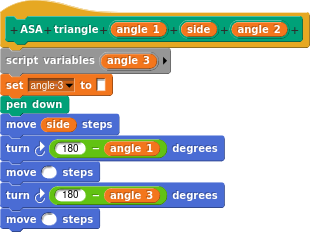
\includegraphics{asaBlockBLANK}
\end{center}
It's your job to use the law of  sines to fill in the blanks. Explain
how you used the law of sines, and show off your work by giving
screenshots of your scripts and stages as provided from \snap.
\begin{freeResponse}
  Ok, to start, note
  \[
  \mathrm{angle~3} = 180 - (\mathrm{angle~1}+\mathrm{angle 2}).
  \]
  Now, 
  \[
  \frac{\mathrm{side}}{\sin(angle~3)} = \frac{\mathrm{first~blank}}{\sin(\mathrm{angle~2})}
  \]
  so
  \[
  \mathrm{first~blank} = \frac{\sin(\mathrm{angle~2})\cdot \mathrm{side}}{\sin(angle~3)}.
  \]
  In a similar way, 
    \[
    \frac{\mathrm{side}}{\sin(angle~3)} = \frac{\mathrm{second~blank}}{\sin(\mathrm{angle~1})}
    \]
    so,
    \[
    \mathrm{second~blank} = \frac{\sin(\mathrm{angle~1})\cdot \mathrm{side}}{\sin(angle~3)}.
    \]
    Here is my Script and my Stage:
    \begin{center}
      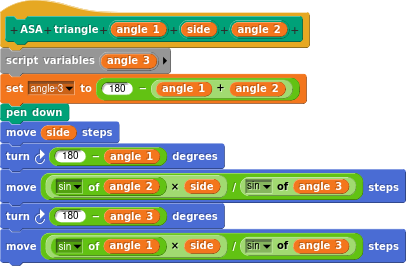
\includegraphics[width=.4\textwidth]{asaBlockCOMPLETE}   \qquad \fbox{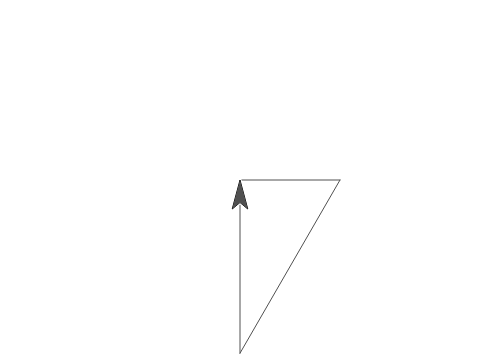
\includegraphics[width=.4\textwidth]{asaStage.png}}
    \end{center}
\end{freeResponse}
\end{question}
\mynewpage

\end{document}